% ----------------------------------------------------------------------
% Date: June 6th, 2024
% Author: Will King
% Project: Chapter 2 - Think Aloud Study
% Document: Presentation for PhD meeting
% ----------------------------------------------------------------------
%
\documentclass[t,compress,9pt,aspectratio=169]{beamer}
\usepackage[english]{babel}
\usepackage[utf8]{inputenc}
\usepackage[nclbghead]{nclbeamer}
\usepackage{listings}
\usepackage{tikz}
\def\checkmark{\tikz\fill[scale=0.4](0,.35) -- (.25,0) -- (1,.7) -- (.25,.15) -- cycle;} 

% Set to 1 or comment to disable transparency and enable full opacity.
\setblockbodyopacity{0.5}

% Listings
\definecolor{cident}{rgb}{0,0.33,0.42}
\definecolor{ckeyw}{rgb}{0,0,0.8}
\definecolor{ccomm}{rgb}{0,0.8,0}
\definecolor{cstr}{rgb}{0.8,0,0}

\lstset{language=[LaTeX]{TeX},
  basicstyle=\footnotesize\ttfamily,
  keywordstyle=\color{ckeyw}\bfseries,
  identifierstyle=\color{cident}\bfseries,
  commentstyle=\color{ccomm},
  stringstyle=\color{cstr},
  showstringspaces=false,
  breaklines=true,
  breakatwhitespace=true,
  tabsize=2,
%   numbers=left,
%   stepnumber=1,
%   firstnumber=1,
%   numberfirstline=true,
  }
  
\nclsetidentity{Faculty of}{Medical Sciences}

\title[NIHR ARC North East and North Cumbria]{\textbf{Valuation of the Weight-Specific Adolescent Instrument for Economic Evaluation using online personal utility functions in an adult population}}
\subtitle{}
\author[King, Will]{Will King \\ \small email: \href{mailto:w.king2@ncl.ac.uk}{w.king2@ncl.ac.uk} \\ \small co-authors: Tom Robinson, Angela Bate, Laura Ternent}
\institute{NIHR ARC North East and
North Cumbria, \\
Newcastle University}
\date[7 October]{7 October, 2024}

% \setlength{\frametitlemargin}{1mm}

\begin{document}
% ==============================================================
%                         --- Welcome frame
% ==============================================================
\begin{frame}[plain]
\maketitle
\end{frame}



% ==============================================================
%                         --- TOC
% ==============================================================
\section*{Presentation structure}
\begin{frame}
\tableofcontents
\frametitle{Presentation structure}
\end{frame}


% ==============================================================
%                         --- Overview
% ==============================================================
\section{Overview}
\begin{frame}[fragile]
\frametitle{Overview}
\begin{itemize}
  \item This presentation will present the methods and results from the valuation of the Weight-Specific Adolescent Instrument for Economic Evaluation (WAItE) using online personal utility functions (OPUF) in a representative sample of UK adults.
  \item Before we dive in...
  \begin{itemize}
      \item What is the WAItE?
      \item What is OPUF?
  \end{itemize}
\end{itemize}
\end{frame}

% ==============================================================
%                         --- Section 1
% ==============================================================
\section{Background}
\begin{frame}[fragile]
\frametitle{Background}
\begin{block}{What is the WAItE?}
    \begin{itemize}
      \item The WAItE is the first weight-specific health related quality of life measure designed for use in adolescents which is appropriate for use in economic evaluation. 
      \item It is composed of 7 attributes and 5 levels (\textit{never, almost never, sometimes, often, always}) within each:
      \begin{itemize}
          \item \textbf{Tired:} I \_\_\_ get tired. %\textit{never, almost never, sometimes, often, always}
          \item \textbf{Walking:} I \_\_\_ struggle to keep up when walking around with others
          \item \textbf{Sports:} I \_\_\_ avoid doing sport
          \item \textbf{Concentration:} I \_\_\_ struggle to concentrate on my studies/work
          \item \textbf{Embarrassment:} I \_\_\_ feel embarrassed shopping for clothes
          \item \textbf{Unhappiness:} I \_\_\_ feel unhappy because I am unable to do the same things as others
          \item \textbf{Treated differently:} People \_\_\_ treat me differently when I go out
      \end{itemize}
    \end{itemize}
\end{block}
\end{frame}


% ==============================================================
%                         --- Section 1
% ==============================================================
\begin{frame}[fragile]
\frametitle{Background}
\begin{block}{What is OPUF?}
    \begin{itemize}
      \item OPUF is a new type of online survey for valuing patient reported outcome measures using more efficient, compositional elicitation methods, which even allow estimating value sets on the individual level. %\cite{Schneider2022TheStates}.
      \item Research has shown that the results are comparable with values estimated via discrete choice experiment.
      \item OPUF main structure:
      \begin{itemize}
          \item Attribute weighting
          \item Level rating
          \item Anchoring task
      \end{itemize}
    \end{itemize}
\end{block}
\end{frame}


% ==============================================================
%                         --- Section 1
% ==============================================================



\section{Aims}
\begin{frame}[fragile]
\frametitle{Aims}
\begin{itemize}
  \item To undertake a population-based valuation survey with adults using the WAItE OPUF to determine their preferences.
  \item To elicit a health state utility value for the WAItE PITS state.
  \item To explore preference heterogeneity within our sample and how it varies among different subgroups.
\end{itemize}
\end{frame}




% Methods
\section{Methods}
\begin{frame}{Methods}
    \frametitle{Methods}
    \begin{block}{Recruitment}
        \begin{itemize}
        \item 300 adults were recruited to respond to a quality-of-life survey hosted online.
        \item Study participants were recruited based on specific quotas to form a representative sample based on UK census data.
        \item The survey was hosted on the \hyperlink{https://www.prolific.com}{Prolific} platform which invited paid respondents to complete the WAItE OPUF survey.
        \item Participation in this survey was estimated to take approximately fifteen minutes to complete and participants received £2.50 as a payment upon completion.
        \end{itemize}
    \end{block}
\end{frame}




% Methods2
\begin{frame}{Survey structure}
    \frametitle{Survey structure}
\begin{itemize}
    \item Consent
    \item WAItE descriptive system   
    \item Attribute weighting: \textit{determine relative importance of the attributes} 
    \item Level rating: \textit{determine importance of levels within each attribute}
    \item Anchoring: \textit{determine the utility value of the worst WAItE health state}
    \item Survey feedback and demographic questions
\end{itemize} 
\end{frame}

\begin{frame}{Utility value estimation}
    \frametitle{Utility value estimation}
    \begin{itemize}
        \item Attribute ratings are normalised to sum to 1 to denote their relative importance.
        \item Attribute weighting is combined with level ratings to yield a coefficient matrix which defines the marginal disutilities associated with each attribute level combination for the WAItE. An example is shown below:
    \end{itemize}
    
\begin{equation}\label{level_matrix}
L_{ij} = 
\begin{bmatrix}
0 & 0 & 0 & 0 & 0 & 0 & 0 \\
0.14 & 0.26 & 0.21 & 0.15 & 0.16 & 0.12 & 0.19 \\
0.57 & 0.55 & 0.63 & 0.54 & 0.38 & 0.26 & 0.66 \\
0.83 & 0.82 & 0.85 & 0.86 & 0.64 & 0.38 & 0.91 \\
1 & 1 & 1 & 1 & 1 & 1 & 1 \\
\end{bmatrix}
\end{equation}
\\
\begin{equation}\label{weight_vector}
w_j = \begin{bmatrix}
    0.08& 0.10& 0.11& 0.14& 0.30& 0.10& 0.17
\end{bmatrix} 
\end{equation}
\\

\begin{equation}\label{eq:element_wise_multiplication}
    L_{ij} \cdot  w_{j} = {\tilde{M}}_{ij}
\end{equation}

\end{frame}

\begin{frame}{Utility value estimation}
    \frametitle{Utility value estimation}
    \begin{itemize}
        \item Combining attribute weightings with level ratings yields coefficient matrix \(\tilde{M}_{ij}\) 
    \end{itemize}
\begin{equation}\label{coeff_matrix}
\tilde{M}_{ij} =  
\begin{bmatrix}
0 & 0 & 0 & 0 & 0 & 0 & 0 \\
0.01 & 0.03 & 0.02 & 0.02 & 0.05 & 0.01 & 0.03 \\
0.05 & 0.05 & 0.07 & 0.07 & 0.11 & 0.03 & 0.11 \\
0.07 & 0.08 & 0.09 & 0.12 & 0.19 & 0.04 & 0.15 \\
0.08 & 0.10 & 0.11 & 0.14 & 0.30 & 0.10 & 0.17
\end{bmatrix}
\end{equation}
\\
    \begin{itemize}
        \item Then anchoring the coefficient matrix using the PITS utility value (\(P = 0.2\)) yields the anchored coefficient matrix \(\tilde{V}_{ij}\) 
    \end{itemize}
\begin{equation}\label{eq:anchoring}
    \tilde{M}_{ij} \cdot (1-P) \quad \backepsilon \quad P = 0.2 
\end{equation}

\begin{equation}\label{ma:anchored_matrix}
\tilde{V}_{ij} =  
\begin{bmatrix}
0 & 0 & 0 & 0 & 0 & 0 & 0 \\
0.01 & 0.02 & 0.02 & 0.02 & 0.04 & 0.01 & 0.02 \\
0.04 & 0.04 & 0.06 & 0.06 & 0.09 & 0.02 & 0.09 \\
0.06 & 0.06 & 0.07 & 0.10 & 0.15 & 0.03 & 0.12 \\
0.06 & 0.08 & 0.09 & 0.11 & 0.24 & 0.08 & 0.14 \\
\end{bmatrix}
\end{equation}
\\

\end{frame}


\begin{frame}{Methods}
    \frametitle{Preference heterogeneity}
    \begin{itemize}
        \item Investigating the heterogeneity of preferences between individuals, required a measure of dis/similarity to quantify how far apart two PUFs are.
        \item A utility value set was estimated for each individual in our sample and euclidean distance (EUD) was used to assess dis/similarity between preferences (shown below).
        \item We then used permutational analysis of variance (PERMANOVA) to explore which factors were influencing preference heterogeneity in our sample.
    \end{itemize}
    
\begin{equation} \label{eq:EUD}
  \begin{aligned}
    d_{EUD}(i,j) & =\sqrt{\sum_{}^{}(u_{i}(s_{1})-u_{j}(s_{1}))^{2}+ ... +(u_{i}(s_{78125})-u_{j}(s_{78125}))^{2}}\\
      & \backepsilon \quad \quad s = \{1111111, 2111111, ..., 5555555\}\\
  \end{aligned}
\end{equation}
\end{frame}


\section{Results}
\begin{frame}{Results}
    \frametitle{Participant Characteristics}
    \begin{table}[h]
    \label{tab:demographicdataadultOPUF}
    \centering
    \begingroup\tiny
    \setlength{\tabcolsep}{2pt} % Reduce space between columns
    \begin{tabular}{p{4cm} p{2cm} p{4cm} p{2cm}} % Split into two sections
    \hline
    \textbf{Characteristic} & \textbf{N (\%)} & \textbf{Characteristic} & \textbf{N (\%)} \\
    \hline
    \textbf{Age} &  & \textbf{Ethnicity} &  \\
    \quad 18-24 & 32 (10.9\%) & \quad White & 251 (84\%) \\
    \quad 25-34 & 50 (17\%) & \quad Asian & 23 (8\%) \\
    \quad 35-44 & 48 (16.3\%) & \quad Black & 11 (4\%) \\
    \quad 45-54 & 49 (16.7\%) & \quad Mixed & 10 (3\%) \\
    \quad 55-64 & 81 (27.6\%) & \quad Other & 5 (2\%) \\
    \quad 65-90 & 34 (11.6\%) & \textbf{Weight Status} & \\
    \quad Not Stated & 6 (2.0\%) & \quad Normal & 154 (51\%) \\
    \textbf{Gender} &  & \quad Overweight & 104 (35\%) \\
    \quad Female & 154 (51\%) & \quad Obese & 30 (10\%) \\
    \quad Male & 144 (48\%) & \quad Underweight & 8 (3\%) \\
    \quad Non-binary & 1 (0\%) & \quad Prefer not to say & 4 (1\%) \\
    \textbf{Education} &  & \quad Underweight & 8 (3\%) \\
    \quad Degree & 147 (49\%) & \quad Prefer not to say & 4 (1\%) \\
    \quad A Level & 64 (21\%) & \textbf{Occupation} &  \\
    \quad Higher Education & 46 (15\%) & \quad Full-time & 130 (43\%) \\
    \quad Other & 20 (7\%) & \quad Part-time & 62 (21\%) \\
    \quad GCSE A-C & 18 (6\%) & \quad Not Paid & 30 (10\%) \\
    \quad GCSE D-G & 5 (2\%) & \quad Other & 31 (10\%) \\
    \textbf{WAItE} & \textbf{Mean (SD)} & \quad Starting a New Job & 3 (1\%) \\
    \quad Tiredness & 3.4 (0.8) &  & \\
    \quad Walking & 2.1 (1.1) & \\
    \quad Sport & 3.3 (1.3) & \\
    \quad Concentration & 2.7 (1.0) & \\
    \quad Embarrassment & 2.2 (1.2) & \\
    \quad Unhappiness & 2.3 (1.0) & \\
    \quad Treated differently & 1.9 (0.9) &  &  \\
    \quad \textbf{Total} & 17.8 (4.8) & & \\
    \hline
    \end{tabular}
    \endgroup
    \end{table}
\end{frame}




\begin{frame}{Results}
    \frametitle{Level ratings}
\centering
\scalebox{0.95}{

\begin{table}[h]
\label{tab:levels_per_domain}
\centering
\tiny
\begin{tabular}{lrrrr}
  \hline
\textbf{Level rating\(^\alpha\)} & \textbf{Mean (SD)} & \textbf{Median (Q1; Q3)} & \textbf{Min} & \textbf{Max} \\
   \hline
   \textbf{Tired} &  &  &  &  \\
    
   %\quad Never & 0 (0)\(^\alpha\) & Median (Q1; Q3) & Min. & Max. \\
   \quad Almost never & 20.3 (23.2) & 10 (5; 25) & 0 & 100 \\
    \quad Sometimes & 36.3 (19.2) & 33.5 (20; 50) & 0 & 100 \\
    \quad Often & 62.2 (23.9) & 70 (50; 80) & 0 & 100 \\
   %\quad Always & 100 (0)\(^\alpha\) & Median (Q1; Q3) & Min. & Max. \\
   \textbf{Walking} &  &  &  &  \\
   %\quad Never & 0 (0)\(^\alpha\) & Median (Q1; Q3) & Min. & Max. \\
   \quad Almost never & 19.4 (21.8) & 10 (6; 21) & 0 & 100 \\
   \quad Sometimes & 37.7 (19.4) & 40 (24; 50) & 0 & 100 \\
   \quad Often & 63 (26.2) & 71 (50; 80) & 0 & 100 \\
   %\quad Always & 100 (0)\(^\alpha\) & Median (Q1; Q3) & Min. & Max. \\
   \textbf{Sports} &  &  &  &  \\
   %\quad Never & 0 (0)\(^\alpha\) & Median (Q1; Q3) & Min. & Max. \\
   \quad Almost never & 16.6 (21) & 10 (5; 20) & 0 & 100 \\
   \quad Sometimes & 29.5 (22) & 25 (10; 45) & 0 & 100 \\
   \quad Often & 49.8 (29.6) & 50.5 (24.5; 75) & 0 & 100 \\
   %\quad Always & 100 (0)\(^\alpha\) & Median (Q1; Q3) & Min. & Max. \\
   \textbf{Concentration} &  &  &  &  \\
   %\quad Never & 0 (0)\(^\alpha\) & Median (Q1; Q3) & Min. & Max. \\
   \quad Almost never & 21.4 (22.1) & 14 (7; 25) & 0 & 100 \\
   \quad Sometimes & 41.6 (20.1) & 40 (25.8; 53.2) & 0 & 100 \\
   \quad Often & 64.5 (26.2) & 73 (50; 80.2) & 0 & 100 \\
   %\quad Always & 100 (0)\(^\alpha\) & Median (Q1; Q3) & Min. & Max. \\
   \textbf{Embarrassment} &  &  &  &  \\
   %\quad Never & 0 (0)\(^\alpha\) & Median (Q1; Q3) & Min. & Max. \\
   \quad Almost never & 16.6 (22.3) & 10 (4; 20) & 0 & 100 \\
   \quad Sometimes & 29.4 (21.6) & 25 (10; 50) & 0 & 100 \\
   \quad Often & 47.9 (30.4) & 50 (20; 75) & 0 & 100 \\
   %\quad Always & 100 (0)\(^\alpha\) & Median (Q1; Q3) & Min. & Max. \\
   \textbf{Unhappiness} &  &  &  &  \\
   %\quad Never & 0 (0)\(^\alpha\) & Median (Q1; Q3) & Min. & Max. \\
   \quad Almost never & 21.1 (22.2) & 13 (6; 25) & 0 & 100 \\
   \quad Sometimes & 41.4 (22.1) & 41.5 (25; 56) & 0 & 100 \\
   \quad Often & 63.6 (28.2) & 75 (50; 85) & 0 & 100 \\
   %\quad Always & 100 (0)\(^\alpha\) & Median (Q1; Q3) & Min. & Max. \\
   \textbf{Treated differently} &  &  &  &  \\
   %\quad Never & 0 (0)\(^\alpha\) & Median (Q1; Q3) & Min. & Max. \\
   \quad Almost never & 20.9 (24.4) & 11 (5; 25) & 0 & 100 \\
   \quad Sometimes & 35.5 (22.8) & 34.5 (19.8; 50) & 0 & 100 \\
   \quad Often & 55.9 (30.6) & 60.5 (31; 80) & 0 & 100 \\
   %\quad Always & 100 (0)\(^\alpha\) & Median (Q1; Q3) & Min. & Max. \\
   \hline
   \multicolumn{2}{l}{\(^\alpha\)Levels \textit{Never} and \textit{Always} were fixed at 0 and 100 respectively} \\   
\end{tabular}
\end{table}
}
\end{frame}



\begin{frame}{Results}
    \frametitle{Attribute weighting and anchoring}
\scalebox{1.5}{
\begin{table}[h]
\label{tab:domain_anchoring}
\centering
\tiny
\begin{tabular}{lrrrr}
\hline
\textbf{OPUF Section} & \textbf{Mean (SD)} & \textbf{Median (Q1; Q3)} & \textbf{Min} & \textbf{Max} \\
\hline
\textbf{Domain weighting} &  &  &  &  \\
  \quad Tired & 76.5 (28.4) & 90 (60; 100) & 1 & 100 \\
  \quad Walking & 65.5 (32.5) & 75 (40; 100) & 0 & 100 \\
  \quad Sports & 42.3 (32.8) & 35 (11; 70) & 0 & 100 \\
  \quad Concentration & 67.9 (30.9) & 80 (44; 99.2) & 0 & 100 \\
  \quad Embarrassment & 40.1 (34.3) & 30 (9; 70) & 0 & 100 \\
  \quad Unhappiness & 70 (31.9) & 80 (50; 100) & 0 & 100 \\
  \quad Treated differently & 52.1 (35.6) & 50 (15.8; 86) & 0 & 100 \\
\textbf{Anchoring} &  &  &  &  \\
  \quad WAItE PITS preferred to death & 87.9\% (32.7\%) & 1 (1; 1) & 0 & 1 \\
  \quad WAItE PITS VAS & -0.025 (5.95) & 0.5 (0.2; 0.8) & -99 & 1 \\
  \quad WAItE PITS Utility Value (winsorized \& imputed) & 0.282 (1.456) & 0.5 (0.2; 0.8) & -14.3 & 1 \\
   \hline
\end{tabular}
\end{table}
}
\end{frame}

\begin{frame}{Results}
    \frametitle{Anchoring distribution}
\begin{itemize}
    \item The distribution of PITS utility values were significantly left skewed (illustrated in the figure below). To mitigate this, winsorization of values which lay in the outer 0.1\% of the distribution was conducted. Missing values were imputed using multiple imputation by chained equations. 
\end{itemize}
\begin{figure}[h]
    \centering
    \includegraphics[width=0.6\linewidth]{hist.png}
    \label{fig:OPUFcensoredpits_hist}
\end{figure}
\end{frame}

\begin{frame}{Results}
    \frametitle{Utility value set}

\centering
\scalebox{0.75}{
\begin{table}[h]
\centering
\label{summary_statistics}
\tiny
\setlength{\tabcolsep}{1.5em} % Adjust the column spacing
\renewcommand{\arraystretch}{1} % Adjust the row height
\begin{tabular}{lcccc}
\hline
\textbf{Dimension level} & \textbf{Mean\(^a\) (95\% CI)\(^b\)} & \textbf{Median (Q1; Q3)} & \textbf{Min} & \textbf{Max} \\
\hline
\textbf{Tired} &  &  &  &  \\
\quad Almost never & 0.029 (0.025; 0.033) & 0.029 (0.027; 0.030) & 0.021 & 0.039 \\
\quad Sometimes & 0.052 (0.047; 0.058) & 0.052 (0.050; 0.054) & 0.041 & 0.063 \\
\quad Often & 0.088 (0.082; 0.094) & 0.088 (0.085; 0.090) & 0.077 & 0.103 \\
\quad Always & 0.140 (0.133; 0.148) & 0.140 (0.137; 0.143) & 0.125 & 0.157 \\
\textbf{Walking} &  &  &  &  \\
\quad Almost never & 0.021 (0.018; 0.024) & 0.021 (0.020; 0.022) & 0.016 & 0.027 \\
\quad Sometimes & 0.045 (0.041; 0.049) & 0.045 (0.043; 0.046) & 0.037 & 0.052 \\
\quad Often & 0.075 (0.069; 0.082) & 0.075 (0.073; 0.077) & 0.064 & 0.087 \\
\quad Always & 0.116 (0.108; 0.124) & 0.115 (0.113; 0.118) & 0.101 & 0.131 \\
\textbf{Sports} &  &  &  &  \\
\quad Almost never & 0.012 (0.010; 0.015) & 0.012 (0.012; 0.013) & 0.009 & 0.017 \\
\quad Sometimes & 0.023 (0.020; 0.025) & 0.023 (0.022; 0.024) & 0.018 & 0.029 \\
\quad Often & 0.038 (0.034; 0.044) & 0.038 (0.037; 0.040) & 0.029 & 0.052 \\
\quad Always & 0.069 (0.063; 0.076) & 0.069 (0.067; 0.071) & 0.058 & 0.084 \\
\textbf{Concentration} &  &  &  &  \\
\quad Almost never & 0.026 (0.023; 0.030) & 0.026 (0.025; 0.028) & 0.019 & 0.034 \\
\quad Sometimes & 0.051 (0.047; 0.055) & 0.051 (0.049; 0.052) & 0.044 & 0.060 \\
\quad Often & 0.080 (0.074; 0.086) & 0.080 (0.078; 0.082) & 0.069 & 0.093 \\
\quad Always & 0.121 (0.114; 0.128) & 0.121 (0.118; 0.123) & 0.107 & 0.138 \\
\textbf{Embarrassment} &  &  &  &  \\
\quad Almost never & 0.012 (0.010; 0.014) & 0.012 (0.011; 0.013) & 0.008 & 0.017 \\
\quad Sometimes & 0.022 (0.019; 0.025) & 0.022 (0.021; 0.023) & 0.016 & 0.027 \\
\quad Often & 0.034 (0.030; 0.038) & 0.034 (0.032; 0.035) & 0.025 & 0.043 \\
\quad Always & 0.061 (0.056; 0.067) & 0.061 (0.059; 0.063) & 0.051 & 0.072 \\
\textbf{Unhappiness} &  &  &  &  \\
\quad Almost never & 0.025 (0.022; 0.029) & 0.025 (0.024; 0.026) & 0.019 & 0.033 \\
\quad Sometimes & 0.054 (0.049; 0.059) & 0.054 (0.052; 0.056) & 0.045 & 0.064 \\
\quad Often & 0.083 (0.076; 0.090) & 0.083 (0.081; 0.086) & 0.070 & 0.101 \\
\quad Always & 0.124 (0.117; 0.133) & 0.124 (0.122; 0.127) & 0.110 & 0.142 \\
\textbf{Treated differently} &  &  &  &  \\
\quad Almost never & 0.019 (0.016; 0.022) & 0.019 (0.017; 0.020) & 0.013 & 0.025 \\
\quad Sometimes & 0.035 (0.030; 0.039) & 0.035 (0.033; 0.036) & 0.026 & 0.043 \\
\quad Often & 0.052 (0.048; 0.057) & 0.052 (0.050; 0.054) & 0.042 & 0.062 \\
\quad Always & 0.087 (0.079; 0.095) & 0.087 (0.084; 0.089) & 0.071 & 0.101 \\
\hline
\multicolumn{5}{l}{\(^a\)Coefficients were anchored using a PITS utility value of 0.282.} \\
\multicolumn{5}{l}{\(^b\)Confidence intervals were estimated from bootstrap resampling with 10,000 iterations.} \\
\end{tabular}
\end{table}
}
   
\end{frame}

\begin{frame}{Results}
    \frametitle{Preference heterogeneity}
\scalebox{0.5}{
\begin{figure}[h]
\centering
\begin{subfigure}{\linewidth}
  \centering
  \includegraphics[width=0.95\linewidth]{plain_plot.png}
\end{subfigure}%
\begin{subfigure}{\linewidth}
  \centering
  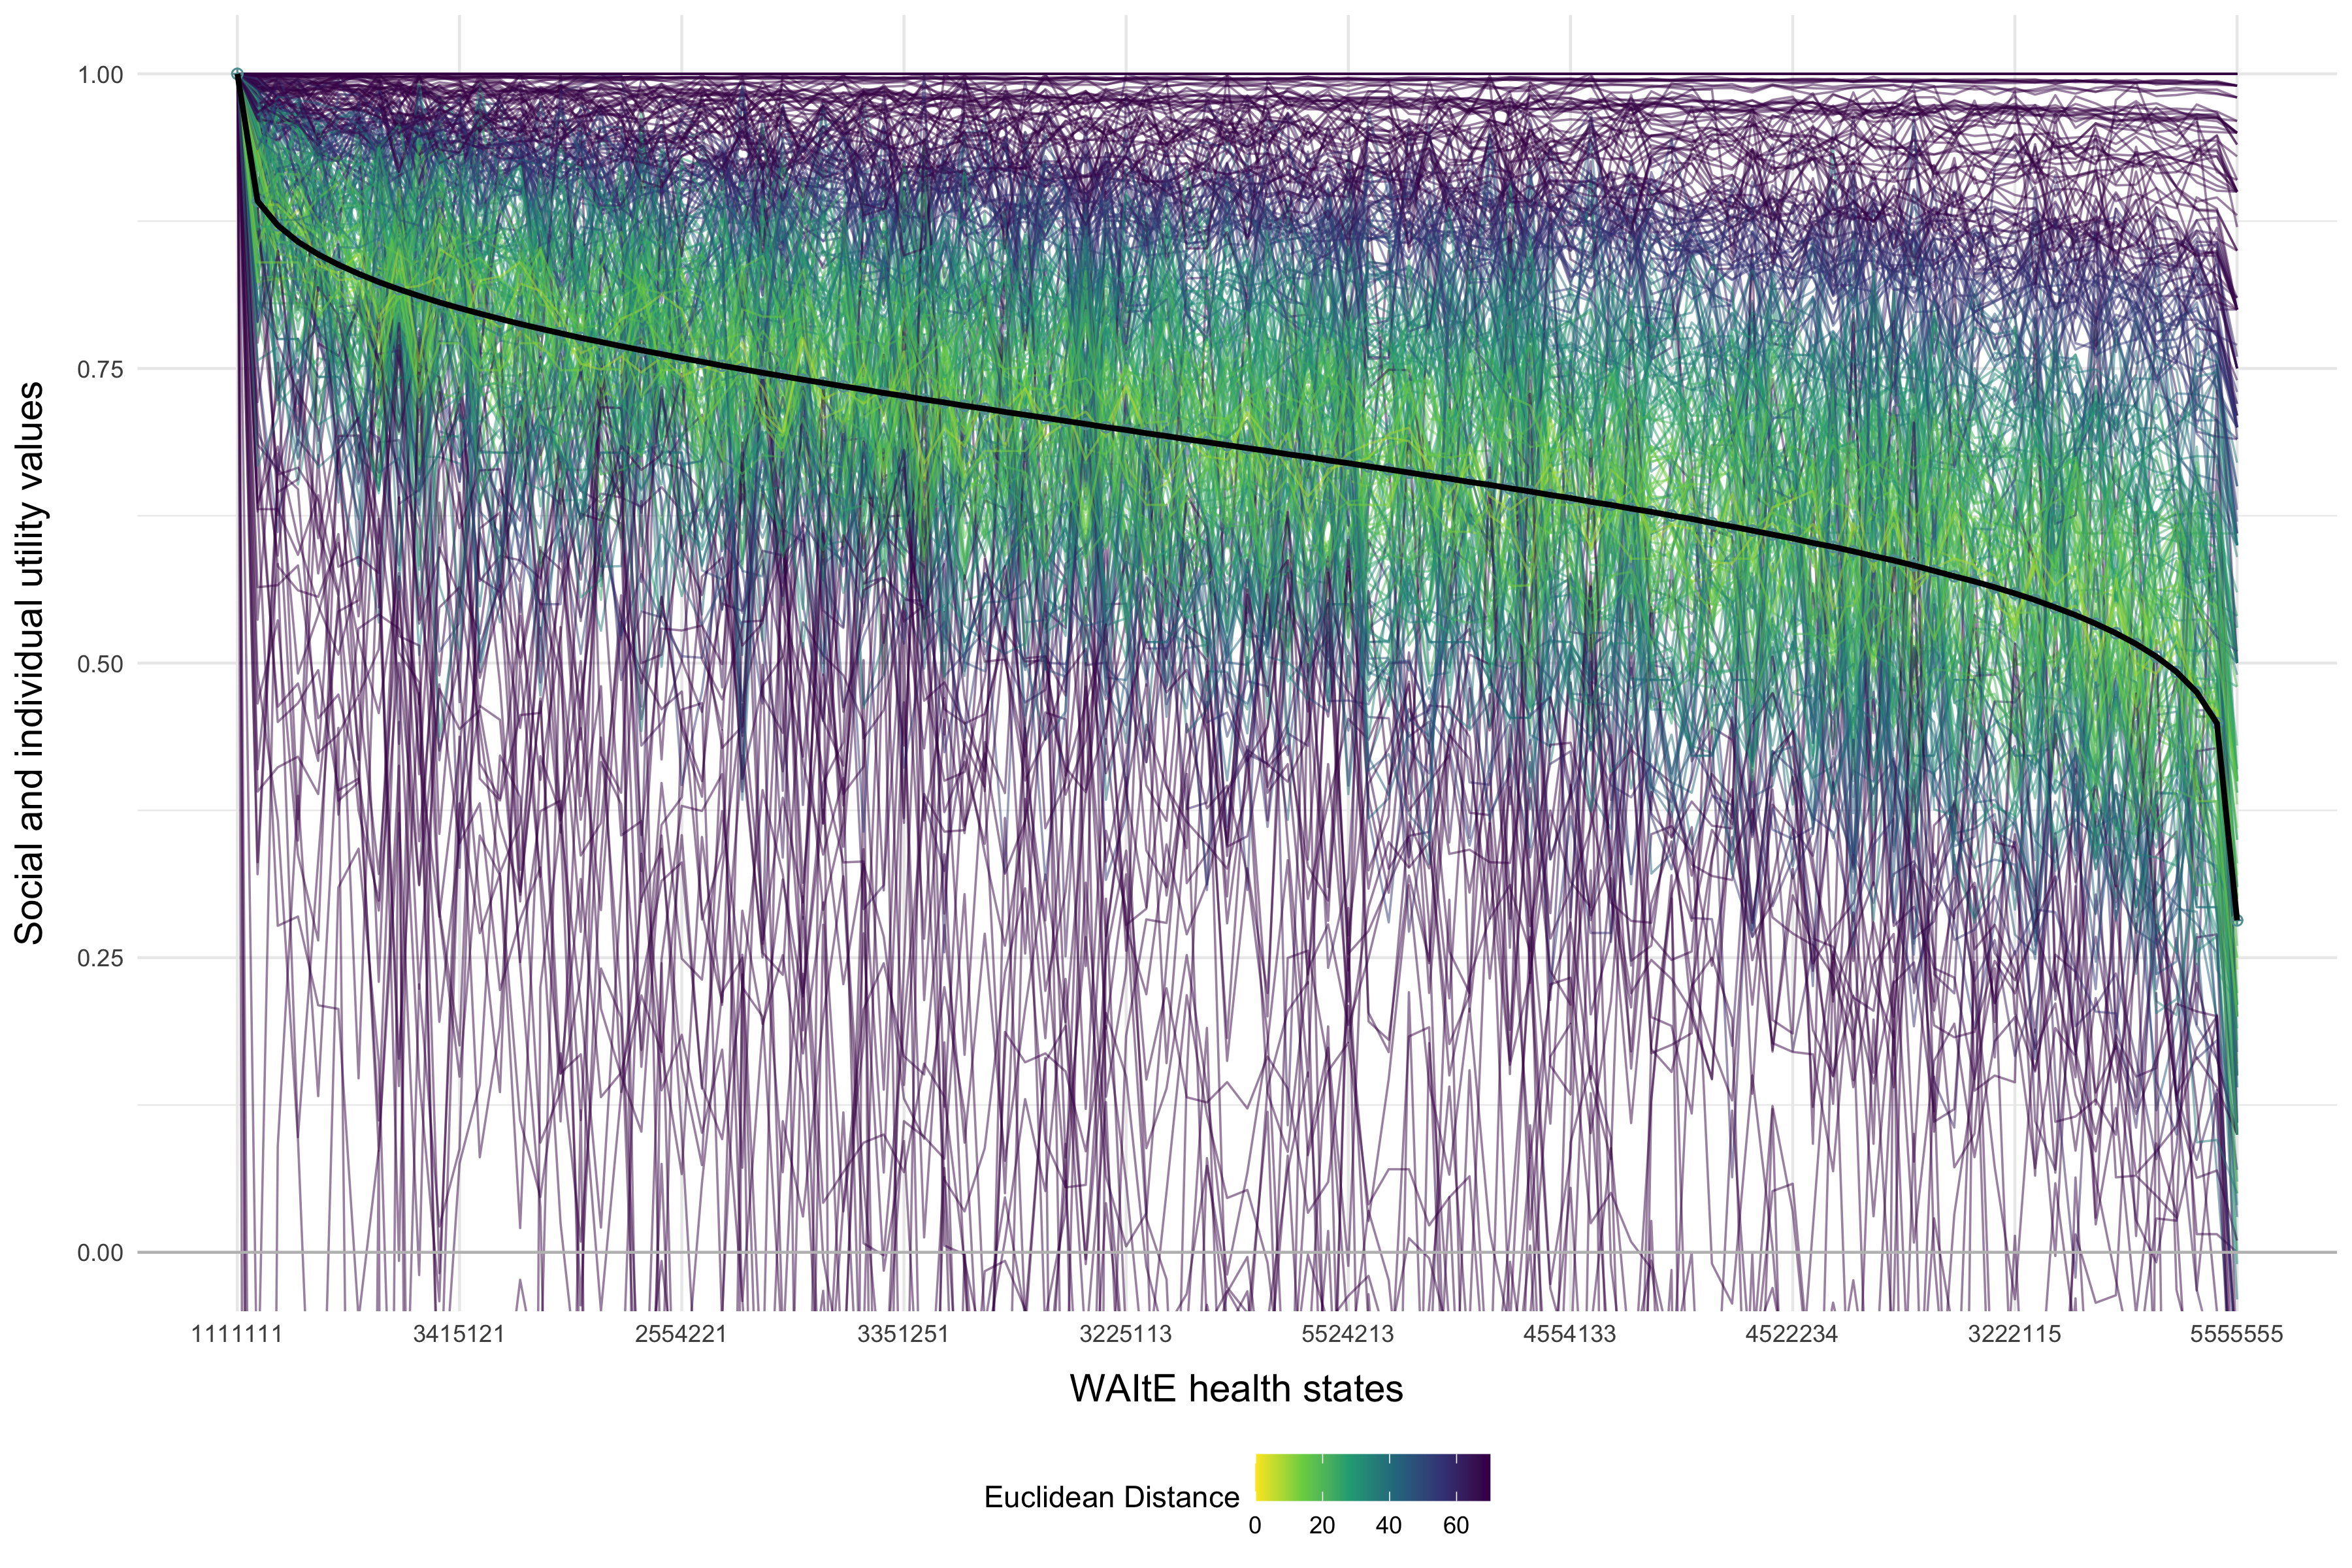
\includegraphics[width=0.95\linewidth]{EUD_plot.png}
\end{subfigure}
\end{figure}
}

\end{frame}



%\begin{figure}[h]
%    \centering
%    \includegraphics[width=0.6\linewidth]{plain_plot.png}
%    \label{fig:individual_group_PUFs}
%\end{figure}

\begin{frame}{Results}
    \frametitle{PERMANOVA}
\scalebox{0.9}{
\begin{table}
\centering
\small
\begin{tabular}{p{7.5cm} p{0.5cm} p{2cm} p{1cm} p{1cm} p{1cm}}
\hline
\textbf{Group variable} & \textbf{Df} & \textbf{SS\(_W\)} & \textbf{R\(^2\)} & \textbf{F} & \textbf{p} \\
\hline
Age & 6 & 663590.648 & 0.057 & 3.018 & 0.030\(^{*}\) \\
Gender & 3 & 57313.577 & 0.005 & 0.521 & 0.362 \\
Weight status & 1 & 6892.412 & 0.001 & 0.188 & 0.727 \\
Education & 5 & 33542.464 & 0.003 & 0.183 & 0.967 \\
Employment status & 7 & 290563.598 & 0.025 & 1.133 & 0.269 \\
Ethnicity & 4 & 521334.829 & 0.045 & 3.557 & 0.056 \\
\hline
Residual & 273 & 10003165.515 & 0.864 &  &  \\
Total (SS\(_T\)) & 299 & 11576403.042 & 1.000 &  & \\
\hline
\multicolumn{6}{l}{Abbreviations: df, degrees of freedom; F, pseudo F statistics; SS\(_T\), total sum‐of‐squares;} \\
\multicolumn{6}{l}{SS\(_W\), within‐group sum‐of‐squares.} \\
\multicolumn{6}{l}{p values based on 10,000 permutations; * = p \(<\) 0.05.}
\end{tabular}
\label{tab:permanova}
\end{table}
}
\end{frame}

\begin{frame}{Results}
    \frametitle{Preference heterogeneity}
    \centering
\scalebox{0.8}{
\begin{figure}[h]
    \centering
    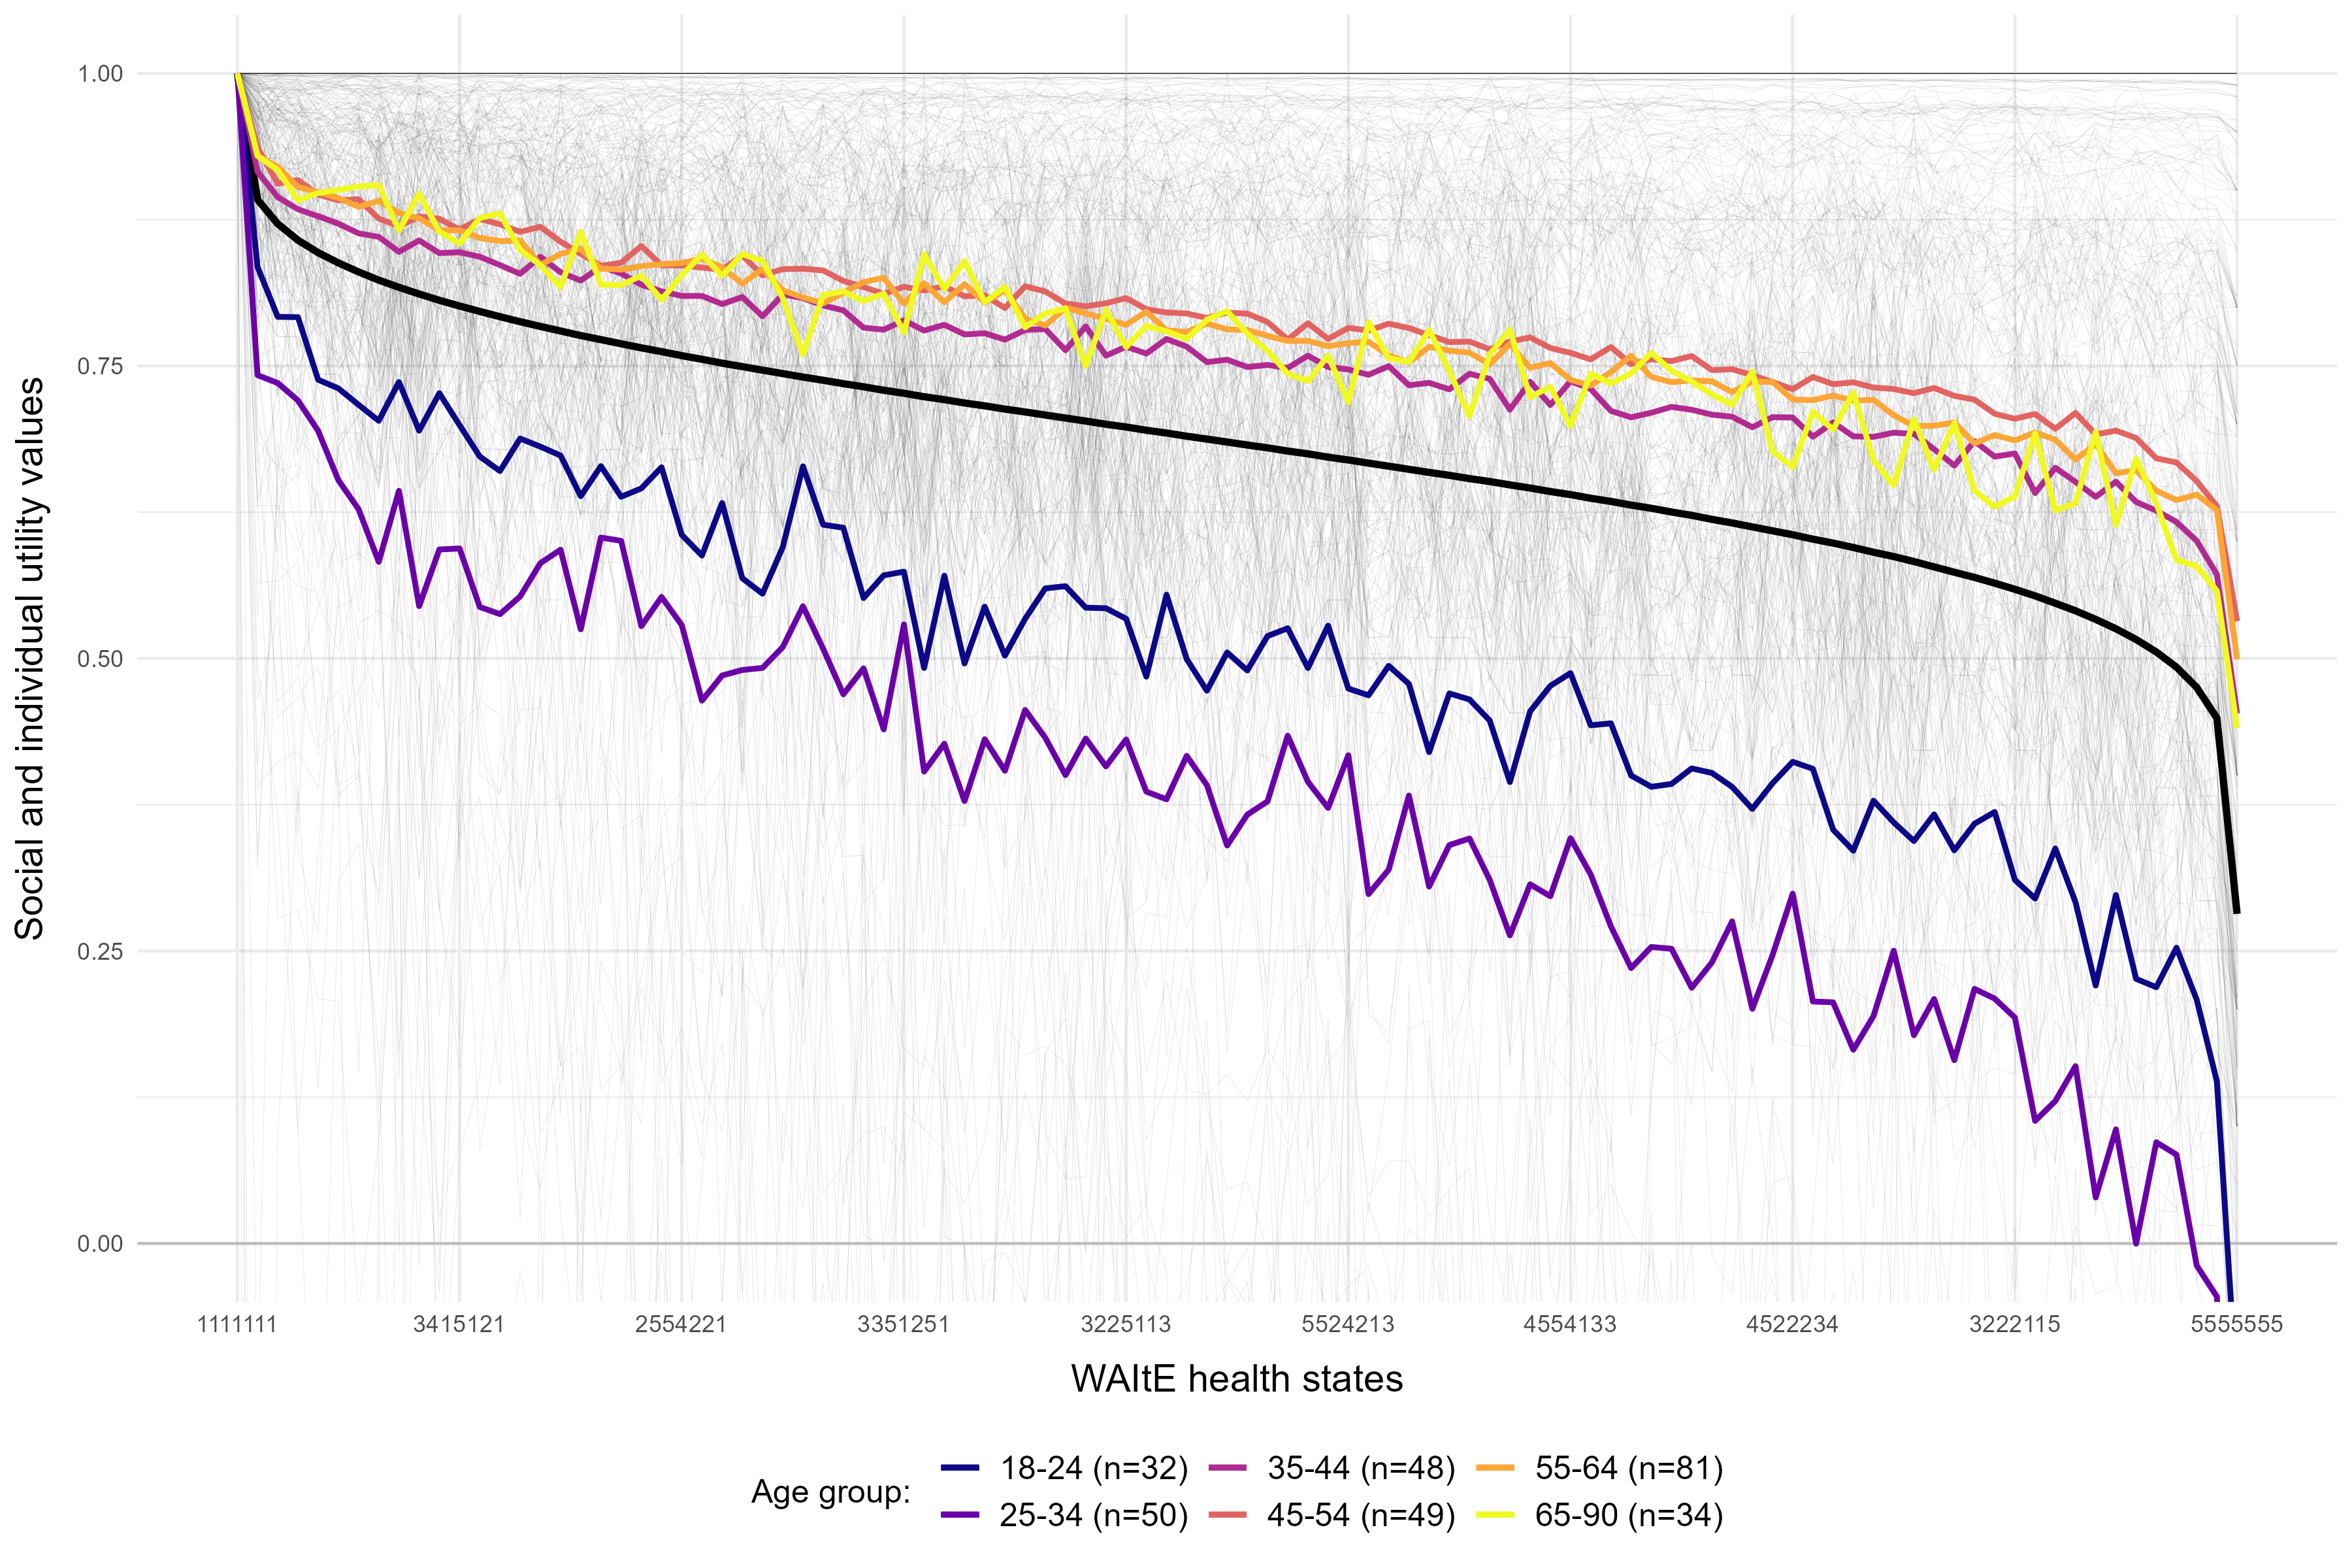
\includegraphics[width=0.8\linewidth]{age_plot.png}
\end{figure}
}

\end{frame}
 


\section{Discussion}
\begin{frame}{Discussion}
    \frametitle{Discussion}
    \begin{itemize}
    \item Tiredness and Unhappiness were considered the most important domains while Embarrassment and Sports the least.
    \begin{itemize}
        \item This was consistent with prior valuation studies that have been completed with the WAItE.
    \end{itemize}
    \item Winsorization limited the effect of outliers on the anchoring factor
    \item EUD and PERMANOVA were used to explore preference heterogeneity and age was shown to have a significant impact on preferences.
    \begin{itemize}
        \item Younger participants generally had lower health state utility values for equivalent health states than older participants. 
    \end{itemize}
    \end{itemize}
\end{frame}

\section{Conclusion}
\begin{frame}{Conclusion}
    \begin{itemize}
        \item Preferences varied significantly by age. This could indicate that adults and adolescents are likely to have systematically different preference values for the same health states. 
        \item Another study in an adolescent population is ongoing to elicit an adolescent valueset for the WAItE using the OPUF.
    \end{itemize}
\end{frame}

% ==============================================================
%                         --- THE END
% ==============================================================
\begin{frame}
\framesingletitle{Thank you for listening}

\end{frame}






% -------------------------------------------------------------
\end{document}

% Version control test 2